

\chapter{Linear Regression}

	\section{Simple Linear Regression}
		We assume the following relationship among the data
		\begin{center}
			$Y \approx \beta_0 + \beta_1X$
		\end{center}
		We regress $Y$ on (onto) $X$
		\begin{center}
			$sales \approx \beta_0 + \beta_1 \times TV$
		\end{center}
		This is a simple \textbf{unvariate model}.
		$\beta_0$, intercept, and $\beta_1$ slope, both are \textbf{coefficients} or \textbf{parameters}.\\
		The estimated value of $Y$ on input $X=x$ is denoted by
		\begin{center}
			$\hat{y} = \hat{\beta}_0 + \hat{\beta}_1 x$
		\end{center}
		\textbf{Given} training data set of $n$ observations
		\begin{center}
			$(x_1,y_1),(x_3,y_2),...,(x_n,y_n)$
		\end{center}
		\textbf{Goal} estimate the unknown coefficients $\beta_0$ and $\beta_1$ such that
		\begin{center}
			$y_i \approx \hat{\beta}_0 + \hat{\beta}_1 x_i$
		\end{center}
		for all $i=1,...,n$ and for future values of $x$.
	
	
	\section{Estimating the Coefficients}
		We We measure deviation of the estimate to the true value by a \textbf{loss function}.
		We mostly use the \textbf{least-squares} function for this purpose.\\
		Let $\hat{y}_i = \hat{\beta}_0 + \hat{\beta}_1 x_i$, then $e_i = y_i - \hat{y}_i$ is the 
		\textbf{residual sum of squares (RSS)}
		\begin{align*}
			RSS &:= e^2_1 + e^2_2 + ... + e^2_n\\
			&= (y_1 - \hat{\beta}_0 + \hat{\beta}_1 x_1)^2 + (y_2 - \hat{\beta}_0 + \hat{\beta}_1 x_2)^2
			+ ... + (y_n - \hat{\beta}_0 + \hat{\beta}_1 x_n)^2
		\end{align*}
		This is a quadratic function in $\beta_0$ and $\beta_1$.
		Setting its derivative to zero yields the least-square coefficient estimates.
		\begin{center}
			$\hat{\beta}_1 = \frac{\sum\limits_{i=1}^m (x_i-\bar{x})(y_i-\bar{y})}{\sum\limits_{i=1}^m (x_i-\bar{x})^2}$
			\ \ \ \ \ \ and\ \ \ \ \ \ 
			$\hat{\beta}_0 = \bar{y} - \hat{\beta}_1\bar{x}$
		\end{center}
		with
		\begin{center}
			\ \ \ \ \ \ \ \ \ 
			$\hat{x} = \frac{1}{n} \sum\limits_{i=1}^n x_i$
			\ \ \ \ \ \ and\ \ \ \ \ \ 
			$\hat{y} = \frac{1}{n} \sum\limits_{i=1}^n y_i$.
		\end{center}
		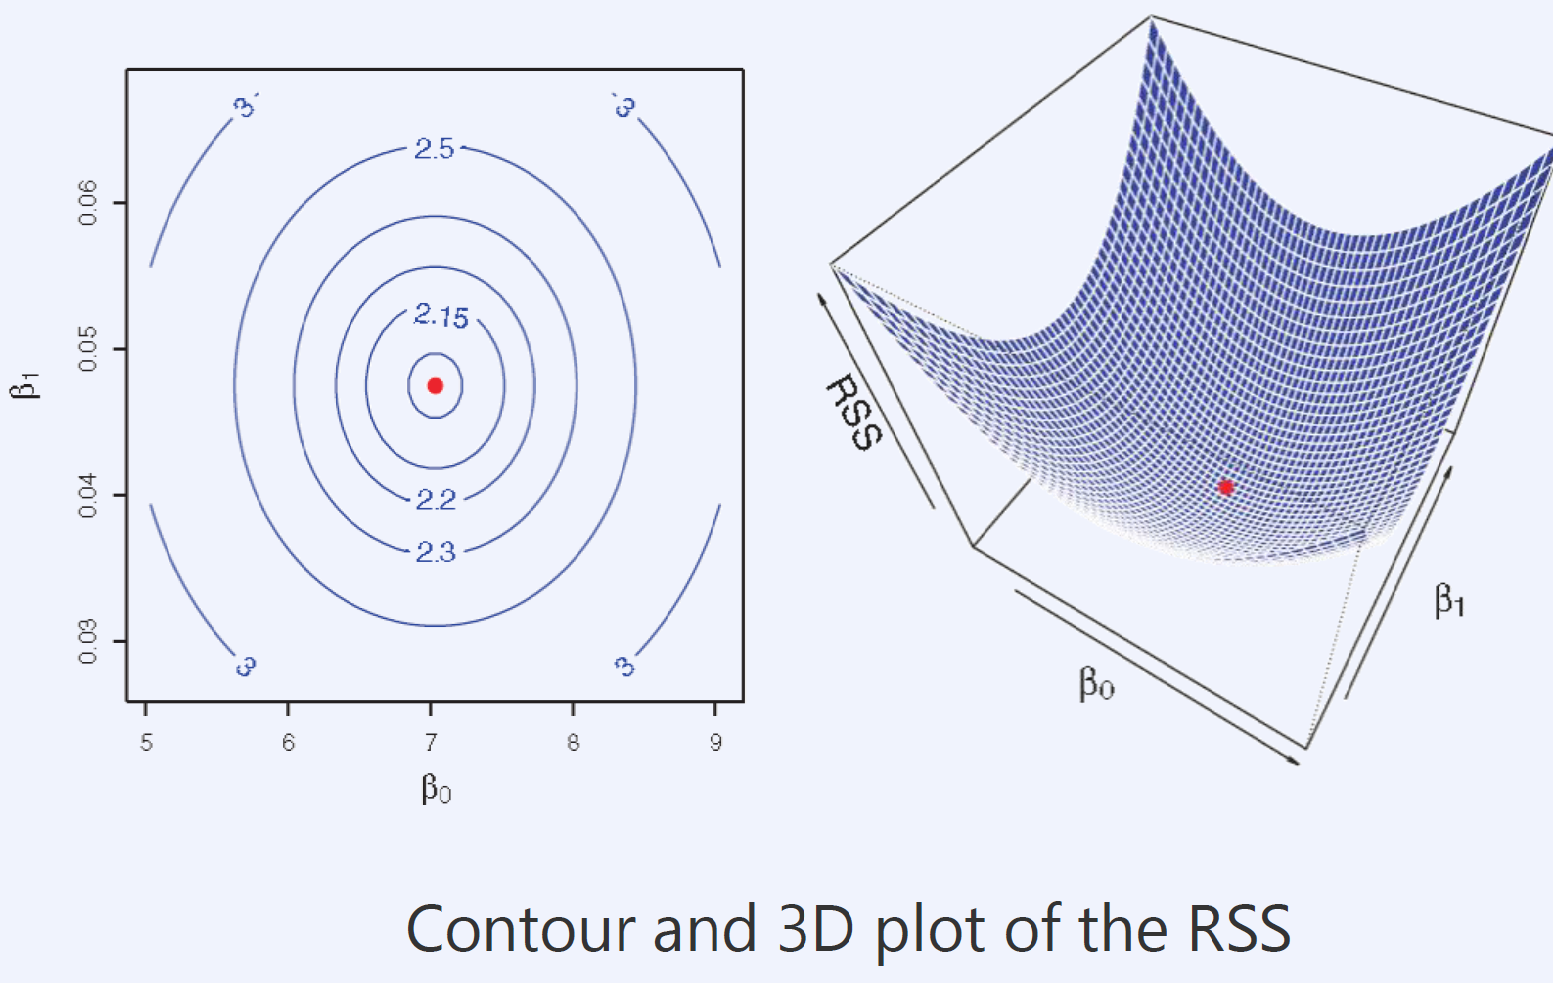
\includegraphics[width=1.05\linewidth]{Graphics/LinearRegression/1.png}
	
	
	\section{Accuracy of Coefficient Estimates}
		We assume the true relationship has an additional noise component that is independent from observations
		\begin{center}
			$Y = \beta_0 + \beta_1X + \epsilon$\ \ \ (*)
		\end{center}
		This is the \textbf{population regression line}, the best linear approximation to the true relationship between $X$ and $Y$, given that the true relationship is (*).
		The population regression line is usually unobserved.\\
		The least-squares fit on the trining data is given by $\hat{y} = \hat{\beta}_0 + \hat{\beta}_1x$.

































